\documentclass[tikz,border=5pt]{standalone}
\usepackage{tikz}
\usetikzlibrary{positioning, fit, arrows.meta, calc, shapes.geometric}

\begin{document}

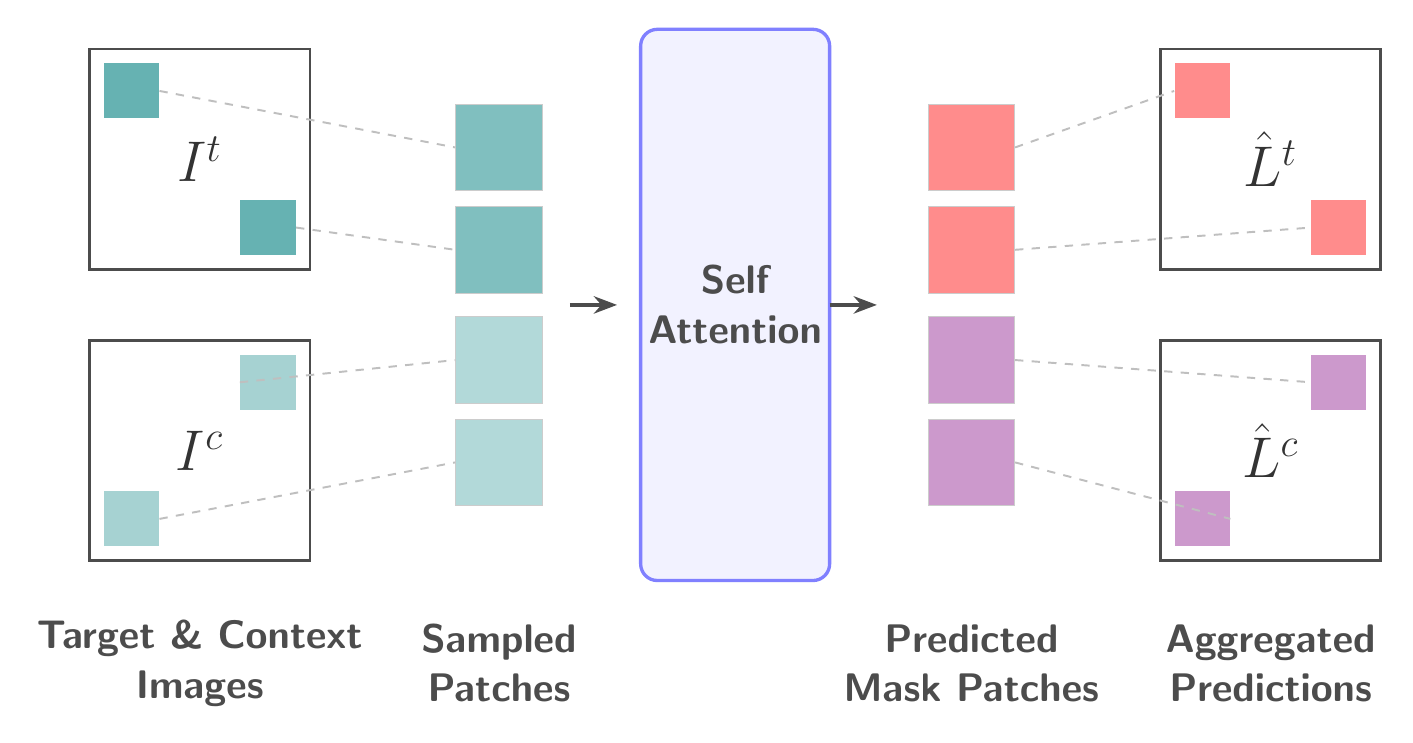
\begin{tikzpicture}[
    font=\sffamily,
    >=Stealth,
    node distance=1.0cm,
    % --- Styles ---
    img_frame/.style={draw=black!70, line width=1pt, fill=white, minimum width=2.8cm, minimum height=2.8cm, inner sep=0pt},
    patch/.style={fill=#1, draw=none, minimum size=0.7cm},
    stack_patch/.style={fill=#1, draw=black!20, line width=0.3pt, minimum size=1.1cm, anchor=center},
    block/.style={draw=blue!50, fill=blue!5, minimum width=2.4cm, minimum height=7.0cm, rounded corners=6pt, align=center, line width=1.2pt},
    arrow_black/.style={->, line width=1.2pt, color=black!70},
    mapping/.style={draw=black!25, dashed, line width=0.7pt},
    label_text/.style={align=center, font=\sffamily\Large\bfseries, color=black!70},
    frame_label/.style={font=\sffamily\huge\bfseries, color=black!80},
]

    % ==========================
    % 1. INPUT IMAGES (Left)
    % ==========================
    \node[img_frame] (It) at (0, 2.2) {};
    \node[frame_label] at (It.center) {$I^t$};
    \node[patch=teal!60] (itp1) at ($(It.north west)+(0.55,-0.55)$) {};
    \node[patch=teal!60] (itp2) at ($(It.south east)+(-0.55,0.55)$) {};

    \node[img_frame] (Ic) at (0, -1.5) {};
    \node[frame_label] at (Ic.center) {$I^c$};
    \node[patch=teal!35] (icp1) at ($(Ic.north east)+(-0.55,-0.55)$) {};
    \node[patch=teal!35] (icp2) at ($(Ic.south west)+(0.55,0.55)$) {};

    \node[label_text] at (0, -4.2) {Target \& Context\\Images};

    % ==========================
    % 2. IMAGE PATCHES STACK
    % ==========================
    \coordinate (stack_pos) at (3.8, 0.35);
    \node[stack_patch=teal!50] (p1) at ($(stack_pos)+(0, 2.0)$) {};
    \node[stack_patch=teal!50] (p2) at ($(stack_pos)+(0, 0.7)$) {};
    \node[stack_patch=teal!30] (p3) at ($(stack_pos)+(0, -0.7)$) {};
    \node[stack_patch=teal!30] (p4) at ($(stack_pos)+(0, -2.0)$) {};

    % Sampling dotted lines
    \draw[mapping] (itp1.east) -- (p1.west);
    \draw[mapping] (itp2.east) -- (p2.west);
    \draw[mapping] (icp1.west) -- (p3.west);
    \draw[mapping] (icp2.east) -- (p4.west);

    \node[label_text] at (3.8, -4.2) {Sampled\\Patches};

    % Arrow 1
    \draw[arrow_black] (4.7, 0.35) -- ++(0.6, 0);

    % ==========================
    % 3. CROSS-ATTENTION BLOCK
    % ==========================
    \node[block] (attn) at (6.8, 0.35) {};
    \node[label_text, font=\sffamily\Large\bfseries] at (attn.center) {Self\\Attention};

    % Arrow 2
    \draw[arrow_black] (8.0, 0.35) -- ++(0.6, 0);

    % ==========================
    % 4. PREDICTED LABEL PATCHES
    % ==========================
    \coordinate (pred_pos) at (9.8, 0.35);
    \node[stack_patch=red!45] (pp1) at ($(pred_pos)+(0, 2.0)$) {};
    \node[stack_patch=red!45] (pp2) at ($(pred_pos)+(0, 0.7)$) {};
    \node[stack_patch=violet!40] (pp3) at ($(pred_pos)+(0, -0.7)$) {};
    \node[stack_patch=violet!40] (pp4) at ($(pred_pos)+(0, -2.0)$) {};

    \node[label_text] at (9.8, -4.2) {Predicted\\Mask Patches};

    % ==========================
    % 5. AGGREGATED OUTPUTS (Right)
    % ==========================
    \node[img_frame] (Lt_pred) at (13.6, 2.2) {};
    \node[frame_label] at (Lt_pred.center) {$\hat{L}^t$};
    \node[patch=red!45] (ltp1) at ($(Lt_pred.north west)+(0.55,-0.55)$) {};
    \node[patch=red!45] (ltp2) at ($(Lt_pred.south east)+(-0.55,0.55)$) {};

    \node[img_frame] (Lc_pred) at (13.6, -1.5) {};
    \node[frame_label] at (Lc_pred.center) {$\hat{L}^c$};
    \node[patch=violet!40] (lcp1) at ($(Lc_pred.north east)+(-0.55,-0.55)$) {};
    \node[patch=violet!40] (lcp2) at ($(Lc_pred.south west)+(0.55,0.55)$) {};

    % Aggregation dotted lines
    \draw[mapping] (pp1.east) -- (ltp1.west);
    \draw[mapping] (pp2.east) -- (ltp2.west);
    \draw[mapping] (pp3.east) -- (lcp1.west);
    \draw[mapping] (pp4.east) -- (lcp2.east);

    \node[label_text] at (13.6, -4.2) {Aggregated\\Predictions};

\end{tikzpicture}
\end{document}